%!TEX root = main.tex

\section{Definitions \& Notation}\label{sec:dfin}

We use the following standard notation: $[n]$ refers to the set of natural numbers $\{1,...,n\}$. Sets are ordinary capital letters $X$, $\sigma$-algebras are script letters $\mathcal{X}$ while random variables are sans serif capitals $\RV{X}:\_\to X$. The calligraphic $\mathcal{G}$ refers to a directed acyclic graph rather than a $\sigma$-algebra. Probability measures are greek letters $\mu,\xi,\gamma$ and stochastic maps are bold capitals $\mathbf{C},\mathbf{H}$. Sets of probability measures or stochastic maps are script capitals: $\mathscr{H}$, $\mathscr{T}$, $\mathscr{J}$. We write the set of all probability measures on $(X,\mathcal{X})$ as $\Delta(\mathcal{X})$ and the set of all stochastic maps $W\to \Delta(X)$ as $\Delta(\mathcal{X})^W$. $\delta_x:\mathcal(X)\to [0,1]$ is the probability measure such that $\delta_x(A)=1$ if $x\in A$ and $0$ otherwise.

If $X$ is a discrete space, probability measures on $X$ are positive row vectors in $\mathbb{R}^{|X|}$ that sum to $1$, and stochastic maps or Markov kernels $X\to \Delta(Y)$ are $|X|\times |Y|$ positive matrices with row sums of 1. Using the standard notion of associative matrix-vector products, given $\mu\in \Delta(X)$ and $\mathbf{A}:X\to \Delta(Y)$, $\mu \mathbf{A}$ is a probability measure on $Y$. Given a random variable (or equivalently, measurable function) $\RV{T}:Y\to Z$, $\mathbf{A} \RV{T}$ is a measurable function $X\to Z$. Given $\mathbf{A}:X\to \Delta(Y)$ and $\mathbf{B}:Y\to \Delta(Z)$, $\mathbf{A}\mathbf{B}$ is a stochastic map $X\to \Delta(Z)$. We can use this same notation for continuous sets $X$ and $Y$, see \citet{cinlar_probability_2011}. 

Write $\mathbf{A}_x$ for the probability measure given by $\delta_x \mathbf{A}$, for $E\subset X$ write $\mathbf{A}_E$ for $\mathbf{A} \mathds{1}_C$ where $\mathds{1}_E$ is the indicator function on $E$, and write $\mathbf{A}(x;E):=A_x(E):=\delta_x A_E$. The tensor product $\mathbf{A}\otimes\mathbf{B}$ is the stochastic map $X\times Y\to \Delta(Y\times Z)$ given by $(x,y)\mapsto \mathbf{A}_x\mathbf{B}_y$.

Product notation is useful for defining composite kernels and probability measures, but sometimes more elaborate constructions are called for. Here we use string diagrams. String diagrams can always be interpreted as a mixture of matrix products and tensor products of Markov kernels, but we introduce kernels with special notation that helps with interpreting the resulting objects. A kernel $\mathbf{A}:X\to \Delta(\mathcal{Y})$ is written $...$, where the input and output wires are associated with the measureable spaces $(X,\mathcal{X})$ and $(Y,\mathcal{Y})$. Probability measures $\mu\in \Delta(\mathcal{X})$ are written $...$ and measurable functions $X\to Y$ are written $...$. For a thorough definition of string diagrams, see \citet{cho_disintegration_2019}.

The identity $\mathrm{Id}_X:X\to \Delta(X)$ is the Markov kernel $x\mapsto \delta_x$, which we represent with a bare wire, leaving the space implicit. The copy map $\splitter{0.1}:X\to \Delta(X\times X)$ is the Markov kernel $x\mapsto \delta_{(x,x)}$. For $\mathbf{A}:X\to \Delta(Y)$ and $\mathbf{B}:X\to \Delta(Z)$, $\splitter{0.1} (A\otimes B) = \sum_{x\in X} A_x \otimes B_x$. The discard map $\stopper{0.1}$ is the Markov kernel $X\to \{*\}$ given by $x\mapsto \delta_*$, where $*$ is a one element set. 

Given $\mu\in\Delta(X),\mathbf{A}:X\to \Delta(Y)$ as before, the joint distribution on $X\times Y$ that might be informally written $P(\RV{X}) P(\RV{Y}|\RV{X})$ is given in string diagram notation as

\begin{align}
\begin{tikzpicture}
\path (0,0) node[dist] (nu) {$\nu$}
+ (0.5,0.15) node (X) {$\RV{X}$}
+(0.5,-0.15) node (Y) {$\RV{Y}$};
\draw ($(nu.east) + (0,0.15)$) -- (X);
\draw ($(nu.east) + (0,-0.15)$) -- (Y);
\end{tikzpicture}
:=\begin{tikzpicture}
\path (0,0) node[dist] (mu) {$\mu$}
++ (1,0) coordinate (copy0)
+ (1.2,0.5) node (X) {$\RV{X}$}
++ (0.5,-0.5) node[kernel] (A) {$\mathbf{A}$}
++(0.7,0) node (Y) {$\RV{Y}$};
\draw (mu)--(copy0);
\draw (copy0) to [bend left] (X);
\draw (copy0) to [bend right] (A) (A) -- (Y);
\end{tikzpicture}\label{eq:jdist}
\end{align}

A string diagram such as \ref{eq:jdist} that is ``capped'' on the left by a probability measure defines a probability space where the sample space is the Cartesian product of the output wires, the measurable sets are the tensor product of the output $\sigma$-algebras and the probability measure is given by the composition of measures in the diagram. The projection map $\pi_X:X\times Y\to X$ is thus a measurable function; following this observation, we overload the notation for the random variable $\RV{X}$ to label wires on the diagram; when used as such, it always refers to the projetion map $\pi_X$. While a random variable technically requires a probability space, we also use this convention for string diagrams representing kernels $X\to \Delta(\mathcal{Y})$ for arbitrary $X,Y$ (such diagrams feature ``free'' wires on the left and right). Using this convention, the measurable function referred to by the wire label $\RV{X}$ is always unambiguous, but we need to define a prior $\xi \in \Delta(\mathcal{X})$ in order for it to have a distribution. 

Finally, if we are given a set of kernels $\{\mathbf{A},\mathbf{B}\}$ where $\mathbf{A}:X\to \Delta(\mathcal{Y})$, $\mathbf{B}:W\to \Delta(\mathcal{Z})$ and a composition defining some kernel $\mathbf{K}:T\to \Delta(\mathcal{U})$ where $T,U$ are each Cartesian products of some subset of of $\{W,X,Y,Z\}$, we can always construct $\mathbf{K}^*:T\to \Delta(\mathcal{W}\otimes\mathcal{X}\otimes\mathcal{Y}\otimes\mathcal{Z})$ by inserting copy maps in appropriate places. Thus if we have \emph{both} a set of kernels and a diagram defining their composition, we can cautiously regard the input and output wires of \emph{each} kernel as a random variable under the same interpretation as given above.

If we regard $\nu$ as a joint distribution of $\RV{X}$ and $\RV{Y}$, the marginal $\nu_{\RV{X}}$, which by definition of $\nu$ is equal to $\mu$, is given by

\begin{align}
\begin{tikzpicture}
\path (0,0) node[dist] (NU) {$\nu$}
+ (0.5,0.15) node (X) {$\RV{X}$}
+(0.5,-0.15) node (Y) {};
\draw ($(NU.east) + (0,0.15)$) -- (X);
\draw[-{Rays [n=8]}] ($(NU.east) + (0,-0.15)$) -- (Y);
\end{tikzpicture}=
\begin{tikzpicture}
\path (0,0) node[dist] (MU) {$\mu$}
+ (0.5,0) node (X) {$\RV{X}$};
\draw (MU) -- (X);
\end{tikzpicture}\label{eq:nu_mu}
\end{align}

A disintegration $\nu_{\RV{Y}|\RV{X}}$ is any kernel $X\to \Delta(\mathcal{Y})$ such that 
\begin{align}
\begin{tikzpicture}
\path (0,0) node[dist] (mu) {$\nu$}
++ (1,0.15) coordinate (copy0)
+ (1.2,0.5) node (X) {$\RV{X}$}
++ (0.5,-0.5) node[kernel] (A) {$\nu_{\RV{Y}|\RV{X}}$}
++(0.7,0) node (Y) {$\RV{Y}$};
\draw ($(mu.east)+(0,0.15)$)--(copy0);
\draw[-{Rays [n=8]}] ($(mu.east) + (0,-0.15)$) -- ($(mu.east) + (0.5,-0.15)$);
\draw (copy0) to [bend left] (X);
\draw (copy0) to [bend right] (A) (A) -- (Y);
\end{tikzpicture}:=
\begin{tikzpicture}
\path (0,0) node[dist] (nu) {$\nu$}
+ (0.5,0.1) node (X) {$\RV{X}$}
+(0.5,-0.1) node (Y) {$\RV{Y}$};
\draw ($(nu.east) + (0,0.1)$) -- (X);
\draw ($(nu.east) + (0,-0.1)$) -- (Y);
\end{tikzpicture}
\end{align}

Disintegrations are known to exist wherever $X$ and $Y$ are standard measurable spaces (ismorphic to a discrete space or the reals with the Borel $\sigma$-algebra), though in general they are not unique. We will use the notation $\nu_{\RV{Y}|\RV{X}}$ to refer to an arbitrary representative of the full set of disintegrations. Note that from Equations \ref{eq:jdist} and \ref{eq:nu_mu} it is clear that $\mathbf{A}$ is a disintegration $\nu_{\RV{Y}|\RV{X}}$. We use disintegrations to represent conditional probability.

The copy map and erase maps have the following properties:

\begin{align}
	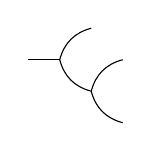
\begin{tikzpicture}[scale=0.8]
	\path (0,0) coordinate (A) 
	++ (0.5,0) coordinate (B)
	+ (0.5,0.5) coordinate (C)
	++ (0.5,-0.5) coordinate (D)
	+(0.5,0.5) coordinate (E)
	+(0.5,-0.5) coordinate (F);
	\draw (A) -- (B);
	\draw (B) to [bend left] (C);
	\draw (B) to [bend right] (D);
	\draw (D) to [bend left] (E);
	\draw (D) to [bend right] (F);
	\end{tikzpicture}
	=
	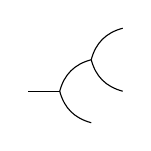
\begin{tikzpicture}[scale=0.8]
	\path (0,0) coordinate (A) 
	++ (0.5,0) coordinate (B)
	+ (0.5,-0.5) coordinate (C)
	++ (0.5,0.5) coordinate (D)
	+(0.5,0.5) coordinate (E)
	+(0.5,-0.5) coordinate (F);
	\draw (A) -- (B);
	\draw (B) to [bend right] (C);
	\draw (B) to [bend left] (D);
	\draw (D) to [bend left] (E);
	\draw (D) to [bend right] (F);
	\end{tikzpicture}
	:=
		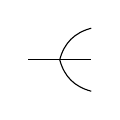
\begin{tikzpicture}[scale=0.8]
	\path (0,0) coordinate (A) 
	++ (0.5,0) coordinate (B)
	+ (0.5,-0.5) coordinate (C)
	+ (0.5,0) coordinate (D)
	+(0.5,0.5) coordinate (E);
	\draw (A) -- (B);
	\draw (B) to [bend right] (C);
	\draw (B) -- (D);
	\draw (B) to [bend left] (E);
	\end{tikzpicture}\label{eq:ccom1}
\end{align}

\begin{align}
	\begin{tikzpicture}[scale=0.8]
	\path (0,0) coordinate (A) 
	++ (0.5,0) coordinate (B)
	+ (0.5,0.5) coordinate (C)
	+ (0.5,-0.5) node (D) {};
	\draw (A) -- (B);
	\draw (B) to [bend left] (C);
	\draw[-{Rays [n=8]}] (B) to [bend right] (D);
	\end{tikzpicture}
	= 
	\begin{tikzpicture}[scale=0.8]
	\path (0,0) coordinate (A) 
	++ (0.5,0) coordinate (B)
	+ (0.5,0.5) node (C) {}
	+ (0.5,-0.5) coordinate (D) ;
	\draw (A) -- (B);
	\draw[-{Rays [n=8]}] (B) to [bend left] (C);
	\draw (B) to [bend right] (D);
	\end{tikzpicture}
	=
	\begin{tikzpicture}[scale=0.8]
	\path (0,0) coordinate (A) 
	++ (1,0) coordinate (B);
	\draw (A) -- (B);
	\end{tikzpicture}\label{eq:ccom2}
\end{align}
And for all $\mathbf{A}$ with appropriate signature
\begin{align}
\begin{tikzpicture}
 \path (0,0) node (A) {}
 ++(0.5,0) node[kernel] (B) {$\mathbf{A}$}
 ++(0.6,0) node (C) {};
 \draw (A.center) -- (B);
 \draw[-{Rays [n=8]}] (B) -- (C);
\end{tikzpicture}
=
\begin{tikzpicture}
 \path (0,0) node (A) {}
  ++(0.5,0) node (C) {};
 \draw[-{Rays [n=8]}] (A.center) -- (C);
\end{tikzpicture}\label{eq:termobj}
\end{align}


A subset of the notation we use for string diagrams is the subject of a coherence theorem: taking a string diagram and applying a planar deformation or any of the rules \ref{eq:ccom1}, \ref{eq:ccom2} and \ref{eq:termobj} yields a string diagram that represents the same kernel \citep{selinger_survey_2010}. This is a key reason for the power of string diagrams.